\documentclass{article}

\newcommand{\logo}{images/PSP-2Color.png}
\usepackage{amsmath, amssymb, amsthm}
\usepackage[letterpaper, margin=1.3in]{geometry}
\usepackage{booktabs}
\usepackage[backend=biber]{biblatex}
\usepackage{caption}
\usepackage[shortlabels]{enumitem}
\usepackage{fancyhdr}
\usepackage{fontspec}
\usepackage{graphicx}
\usepackage{hyperref}
\usepackage{multicol}
\usepackage{pgfplots}
\usepackage{setspace}
\usepackage{siunitx}
\usepackage{tabularray}
\usepackage{tabularx}
\usepackage{tikz}
\usepackage{titlesec}
\usepackage{xcolor}
\usepackage{xparse}

\definecolor{night-sky}{RGB}{37,37,38}
\definecolor{rush}{RGB}{218,170,0}
\definecolor{moondust}{RGB}{242,239,233}

\definecolor{boilermaker-gold}{RGB}{207,185,145}
\definecolor{aged}{RGB}{142,111,62}
\definecolor{field}{RGB}{221,185,69}
\definecolor{dust}{RGB}{235,217,159}
\definecolor{steel}{RGB}{85,89,96}
\definecolor{cool-gray}{RGB}{111,114,123}
\definecolor{railway-gray}{RGB}{157,151,149}
\definecolor{steam}{RGB}{196,191,192}

\setmainfont{Libre Franklin}
\setlength{\parskip}{1.5ex}
\setlength{\parindent}{0.7cm}
\titlespacing\section{0pt}{5pt}{0pt}
\titlespacing\subsection{0pt}{4pt}{0pt}
\titlespacing\subsubsection{0pt}{2pt}{0pt}
\AddToHook{cmd/section/before}{\clearpage}

% TODO: fix this
%\setlength{\headheight}{32.50275pt}
%\addtolength{\topmargin}{-20.50275pt}

\setlist{nosep}

\newfontfamily\titlefont[SizeFeatures={Size=36}]{Saira}
\newfontfamily\titlefontmedium[SizeFeatures={Size=22}]{Saira}
\newfontfamily\titlefontsmall[SizeFeatures={Size=14}]{Saira}
\newcommand{\totitlefont}{\fontsize{36pt}{40pt}\selectfont\titlefont}
\newcommand{\totitlefontmedium}{\fontsize{22pt}{26pt}\selectfont\titlefontmedium}
\newcommand{\totitlefontsmall}{\fontsize{14pt}{16pt}\selectfont\titlefontsmall}

\pgfplotsset{compat=1.18}

\addtolength{\headsep}{1ex}
\renewcommand{\headruleskip}{-1.5ex}
\renewcommand{\headrule}{{\color{rush}\rule{\textwidth}{1pt}}}
\renewcommand{\footrule}{{\color{rush}\rule{\textwidth}{1pt}}}
\renewcommand{\sectionmark}[1]{\markright{#1}}
\renewcommand{\subsectionmark}[1]{}

\addtolength{\abovecaptionskip}{-0.4cm}

\fancypagestyle{toc}{%
    \fancyhf{}%
    \fancyhead[R]{\includegraphics[height=1cm]{\logo}}%
    \fancyfoot[C]{\textbf{\thepage}}%
}

\fancypagestyle{regular}{%
    \fancyhf{}%
    \fancyhead[L]{\textit{\rightmark}}%
    \fancyhead[R]{\includegraphics[height=1cm]{\logo}}%
    \fancyfoot[C]{\textbf{\thepage}}%
}

\hypersetup{
    colorlinks,
    linkcolor={black},
    citecolor={black},
    urlcolor={blue!70!black}
}

\NewDocumentCommand{\makebasictitlepage}{ O{} m o }{
    \thispagestyle{empty}
    ~ \vspace{2.5cm}

    \begin{center}
        \includegraphics[width=9cm]{\logo}
    \end{center}
    \vfill

    \setstretch{2.5}

    \noindent {\totitlefont \color{aged} PSP #1}

    \noindent {\totitlefontmedium #2}

    \IfNoValueF{#3}{
        \vspace{-2.5ex}
        \noindent {\totitlefontsmall \color{cool-gray} #3}
    }

    \setstretch{1}

    \vspace{1cm}
    \newpage
}


\addbibresource{bib.bib}

\usepackage{lipsum} % FIXME: testing only

\begin{document}
    \makebasictitlepage[High Altitude]{System Requirements Review and \\ Conceptual Design Review}[December 2022]

    \newpage
    \pagestyle{toc}
    \setstretch{0.9}
    \tableofcontents

    \listoffigures
    \listoftables

    \newpage
    \pagestyle{regular}
    \setstretch{1.2}

    \section{Introduction}
    \lipsum[10]

    \begin{figure}
        \begin{center}
            This is a figure

            \includegraphics[width=0.4\textwidth]{\logo}
        \end{center}
        \caption[Short caption]{Long caption.}
        \label{fig:figure}
    \end{figure}

    \begin{table}
        \begin{center}
            \begin{tabular}{lrr}
                \toprule
                & \multicolumn{2}{c}{Rocket Statistics} \\
                \cmidrule{2-3}
                Rocket Name & Rocket Height (\si{\meter}) & Launch Altitude (\si{\kilo\meter}) \\
                \midrule
                Not a Rocket & 3.1 & 2.2 \\
                This is a Real Rocket & 1.3 & 0.8 \\
                \bottomrule
            \end{tabular}
        \end{center}
        \caption{Caption}
        \label{tab:table}
    \end{table}

    \begin{figure}
        \begin{center}
            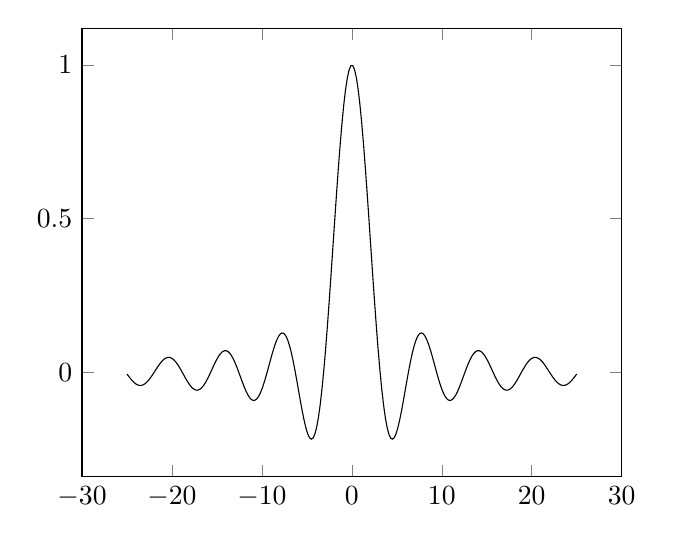
\begin{tikzpicture}
                \begin{axis}
                    \addplot[domain={-25:25}, samples=250] {sin((180/pi) * x) / x};
                \end{axis}
            \end{tikzpicture}
        \end{center}
        \caption{Example plot}
    \end{figure}

    Now we can talk about \autoref{fig:figure}. And, \autoref{tab:table}. \autocite[2]{rocket-paper}
    
    \lipsum[10]
    \lipsum[10]

    \begin{enumerate}
        \item A
        \begin{enumerate}
            \item Nested
            \begin{enumerate}
                \item And more
            \end{enumerate}
        \end{enumerate}
        \item B
        \item C
    \end{enumerate}

    \begin{itemize}
        \item Blah
        \begin{itemize}
            \item more
            \begin{itemize}
                \item and more
            \end{itemize}
        \end{itemize}
        \item \lipsum[5]
        \item abc
        \item def
    \end{itemize}

    \subsection{Intro Subsection}
    \lipsum[10]
    \lipsum[10]
    \lipsum[10]

    \lipsum[10]
    \lipsum[10]
    \lipsum[10]

    \lipsum[10]
    \lipsum[10]
    % \lipsum[10]

    \section{Avionics}
    \lipsum[10]

    \subsection{Avionics subsection}
    \lipsum[10]

    \subsubsection{Avionics sub-subsection}
    \lipsum[10]

    \lipsum[10]
    \lipsum[10]
    \lipsum[10]

    \section{Propulsion}
    \lipsum[10]
    \lipsum[10]
    \lipsum[10]

    \lipsum[10]
    \lipsum[10]
    \lipsum[10]

    \lipsum[10]
    \lipsum[10]
    \lipsum[10]

    \newpage
    \printbibliography
\end{document}
